\documentclass[a4paper,12pt,titlepage]{article}
\usepackage[utf8]{inputenc}
\usepackage{graphicx} % Required for inserting images
\usepackage[spanish,es-tabla]{babel}
\usepackage[none]{hyphenat}
\usepackage[justification=centering]{caption}
\usepackage{subcaption}
\usepackage{amssymb, amsmath}
\usepackage{gensymb}
\usepackage{fancyhdr}

\lhead{Instrumentación electrónica}
\rhead{Gonzalo Bastos González}


%opening
\pagestyle{fancy}

\title{Instrumentación electrónica}
\author{Gonzalo Bastos González}
\date{77543085B}

\begin{document}

\maketitle

\tableofcontents
\newpage

\section{Corriente continua}
\subsection{Objetivos}
    \begin{itemize}
        \item Uso del polímetro para realizar mediciones
        \item Interpretación del código de colores para determinar el valor de las resistencias
        \item Comprobación de la ley de Ohm y de las leyes que rigen el funcionamiento de las resistencias a partir de los datos experimentales
    \end{itemize}

\subsection{Materiales y metodología}
    \begin{itemize}
        \item Placa base y cables de conexión
        \item Polímetro
        \item Resistencias (2)
        \item Fuente de alimentación de corriente continua
    \end{itemize}

El primer paso de nuestra práctica es obtener el valor de nuestras dos resistencias, tanto interpretando su código de colores como midiéndolos experimentalmente. El código de colores debe interpretarse a partir de una tabla como la siguiente:

\begin{figure}[h!]
    \centering
    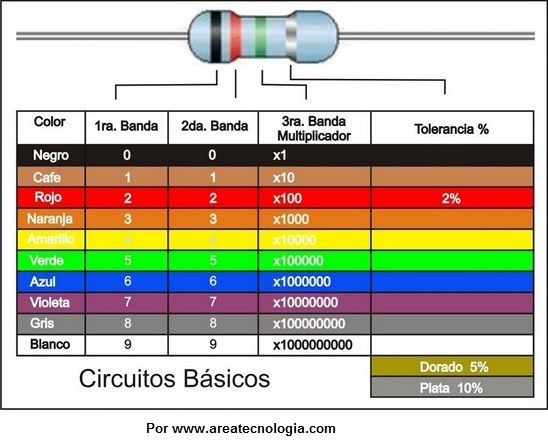
\includegraphics[width=0.6\linewidth]{continua/codigo-colores-resistencias.jpg}
    \caption{Código de colores de una resistencia}
    \label{Codigo de colores}
\end{figure}
\newpage
A continuación debemos comprobar los valores teóricos de las resistencias experimentalmente, conectándolas al polímetro y midiendo su valor, como se muestra en la Fig.\ref{MedidaResistencias}. El valor medido debería estar dentro del margen de tolerancia que indica el código de colores.

\begin{figure}[h!]
    \centering
    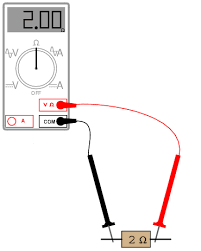
\includegraphics[width=0.3\linewidth]{continua/medidaResistencias.png}
    \caption{Procedimiento experimental para la medida de una resistencia con el polímetro}
    \label{MedidaResistencias}
\end{figure}

\par El otro método que usaremos para comprobar el valor de las resistencias consistirá en una medida indirecta, valiéndonos de la ley de Ohm \newline $(V=IR)$. Mediremos las diferentes intensidades de corriente que producen diferentes valores de voltaje. El valor de la resistencia lo obtendremos a partir de un ajuste por mínimos cuadrados. Para llevar a cabo nuestras mediciones construiremos un circuito simple con la resistencia $R_{1}$ como el siguiente:

\begin{figure}[h!]
    \centering
    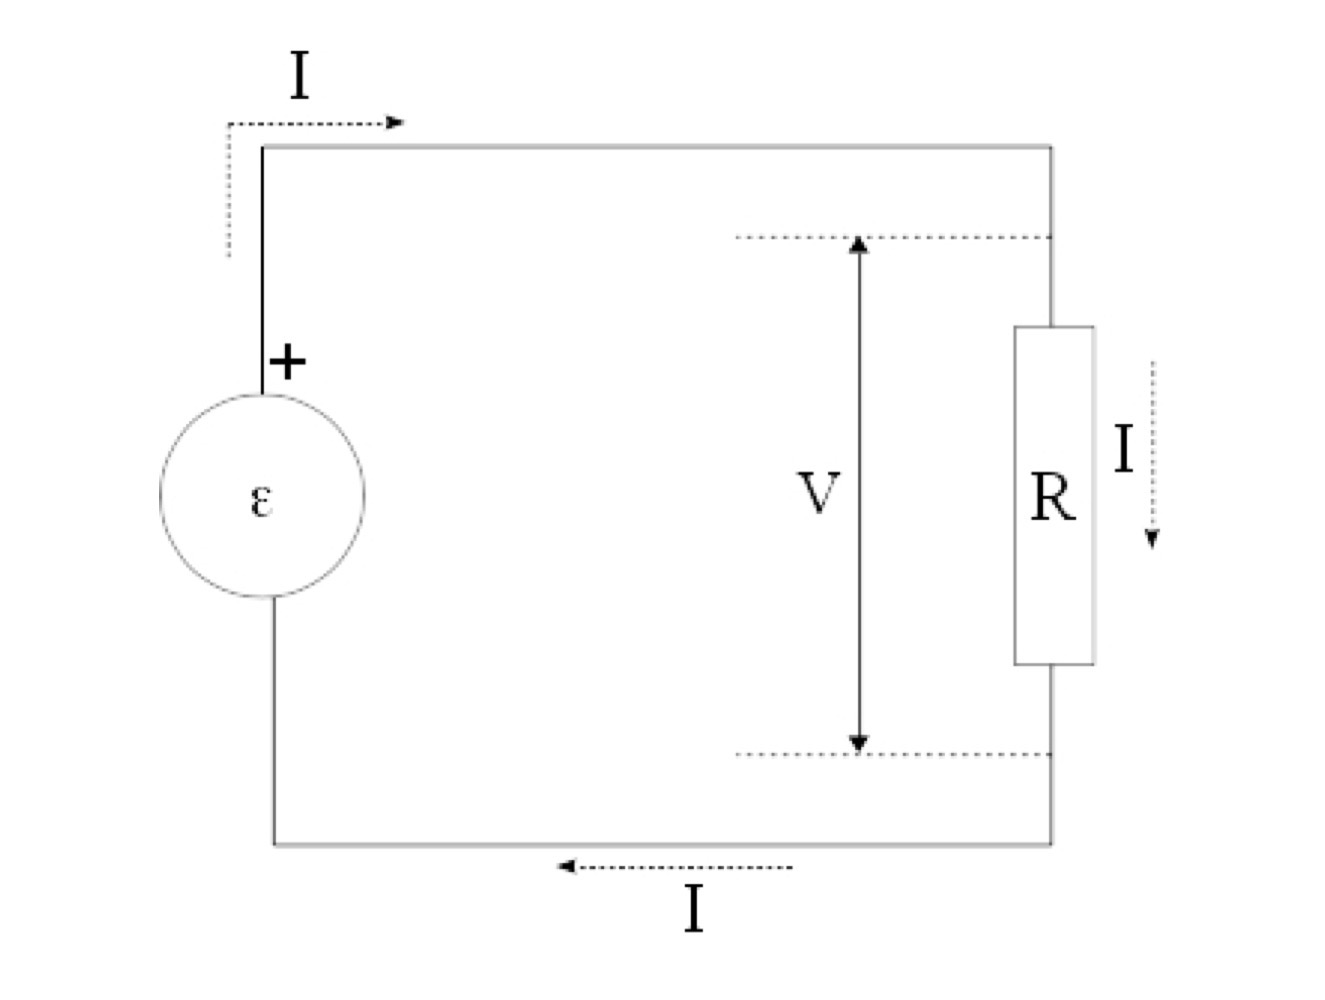
\includegraphics[width=0.5\linewidth]{continua/circuitosimple.jpg}
    \caption{Esquema del circuito simple}
    \label{Circuito simple}
\end{figure}

Para la medida de los potenciales debemos conectar el polímetro en paralelo al circuito, es decir simplemente conectaremos los bornes al elemento del circuito que queremos medir. No obstante, para la medida de las intensidades debemos conectar el polímetro en serie, toda la intensidad debe circular por él, integrando al propio polímetro dentro del circuito.\newline


\par La última parte de la práctica consiste en comprobar las diferencias en el cálculo de resistencias para un circuito en serie y otro en paralelo:

\begin{itemize}
    \item El primer caso que vamos a analizar es el de las resistencias en serie, para ello crearemos un circuito con dos resistencias asociadas en serie como el de la Fig.\ref{CircuitoSerie}. El valor total de la resistencia del circuito es equivalente a un circuito con una sola resistencia que tenga como valor la suma de todas las $R_{i}$, es decir:
        \begin{equation}
            R_{S}=\sum_{k=1}^NR_{k}
        \end{equation}
        Por otra parte, la intensidad de corriente que circula por las resistencias es la misma en ambas, mientras que la ddp (diferencia de potencial) en bornes del conjunto de resistencias cumple lo siguiente:
        \begin{equation}
            V=V_{1}+V_{2}
            \label{Formula V serie}
        \end{equation}
        Siendo $V_{1}$ y $V_{2}$ las ddp de $R_{1}$ y $R_{2}$ respectivamente.
        \begin{figure}[h!]
            \centering
            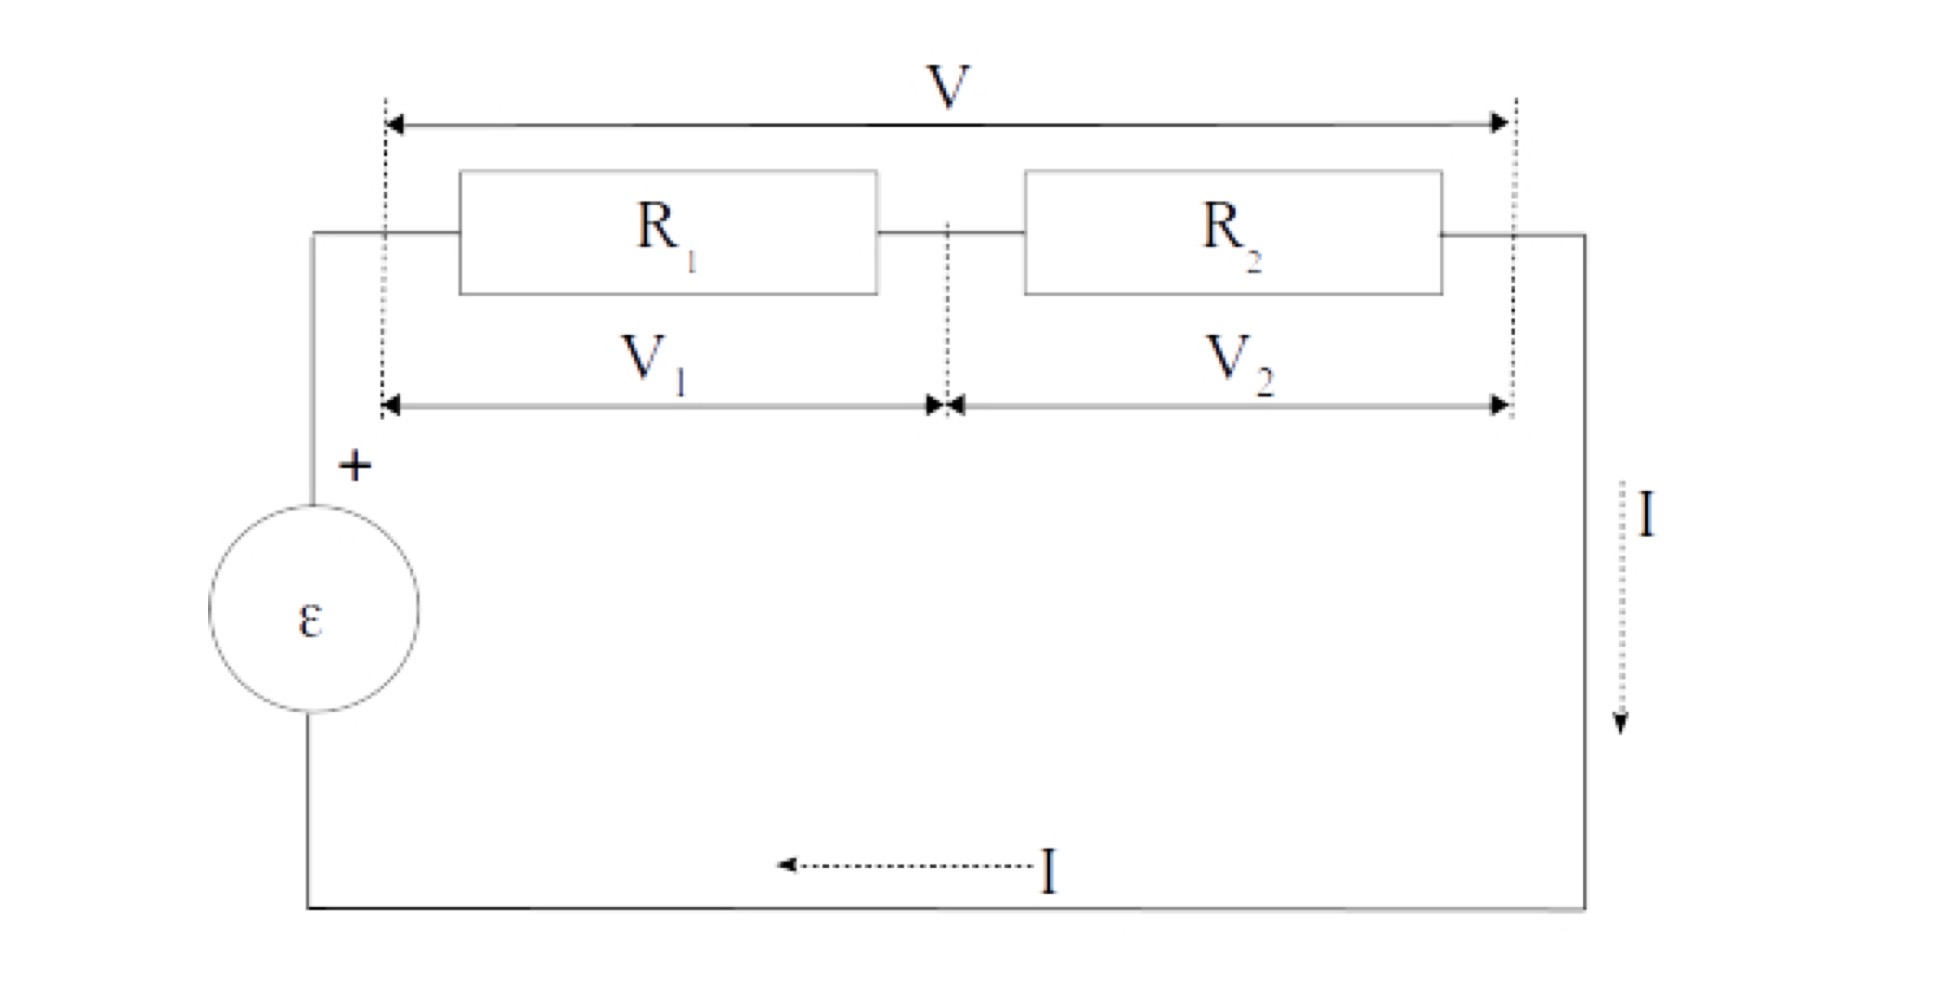
\includegraphics[width=0.8\linewidth]{continua/circuitoserie.jpg}
            \caption{Esquema del circuito de resistencias asociadas en serie}
            \label{CircuitoSerie}
        \end{figure}
    
    \par La medida de las resistencias se va a realizar por dos métodos; de forma directa, conectando el polímetro al circuito y midiendo el valor de la resistencia total, y de forma indirecta, de un modo parecido al del circuito simple, valiéndonos de la ley de Ohm y realizando un ajuste por mínimos cuadrados.
    
    \item El segundo caso que vamos a estudiar es el de un circuito de dos resistencias asociadas en paralelo, para ello crearemos un circuito como el de la Fig.\ref{CircuitoParalelo}. El valor total de la resistencia del circuito tiene la siguiente expresión:
    \begin{equation}
        \frac{1}{R_{P}}=\sum_{k=1}^N\frac{1}{R_{k}}
        \label{Resistencias en paralelo}
    \end{equation}
    Por otra parte la ddp de potencial en bornes de cada resistencia es la misma y las intensidades de corriente cumplen la siguiente relación:
    \begin{equation}
        I=I_{1}+I_{2}
        \label{Formula I paralelo}
    \end{equation}
    siendo $I_{1}$ y $I_{2}$ las intensidades que circulan por $R_{1}$ y $R_{2}$ respectivamente.
    \begin{figure}[h!]
        \centering
        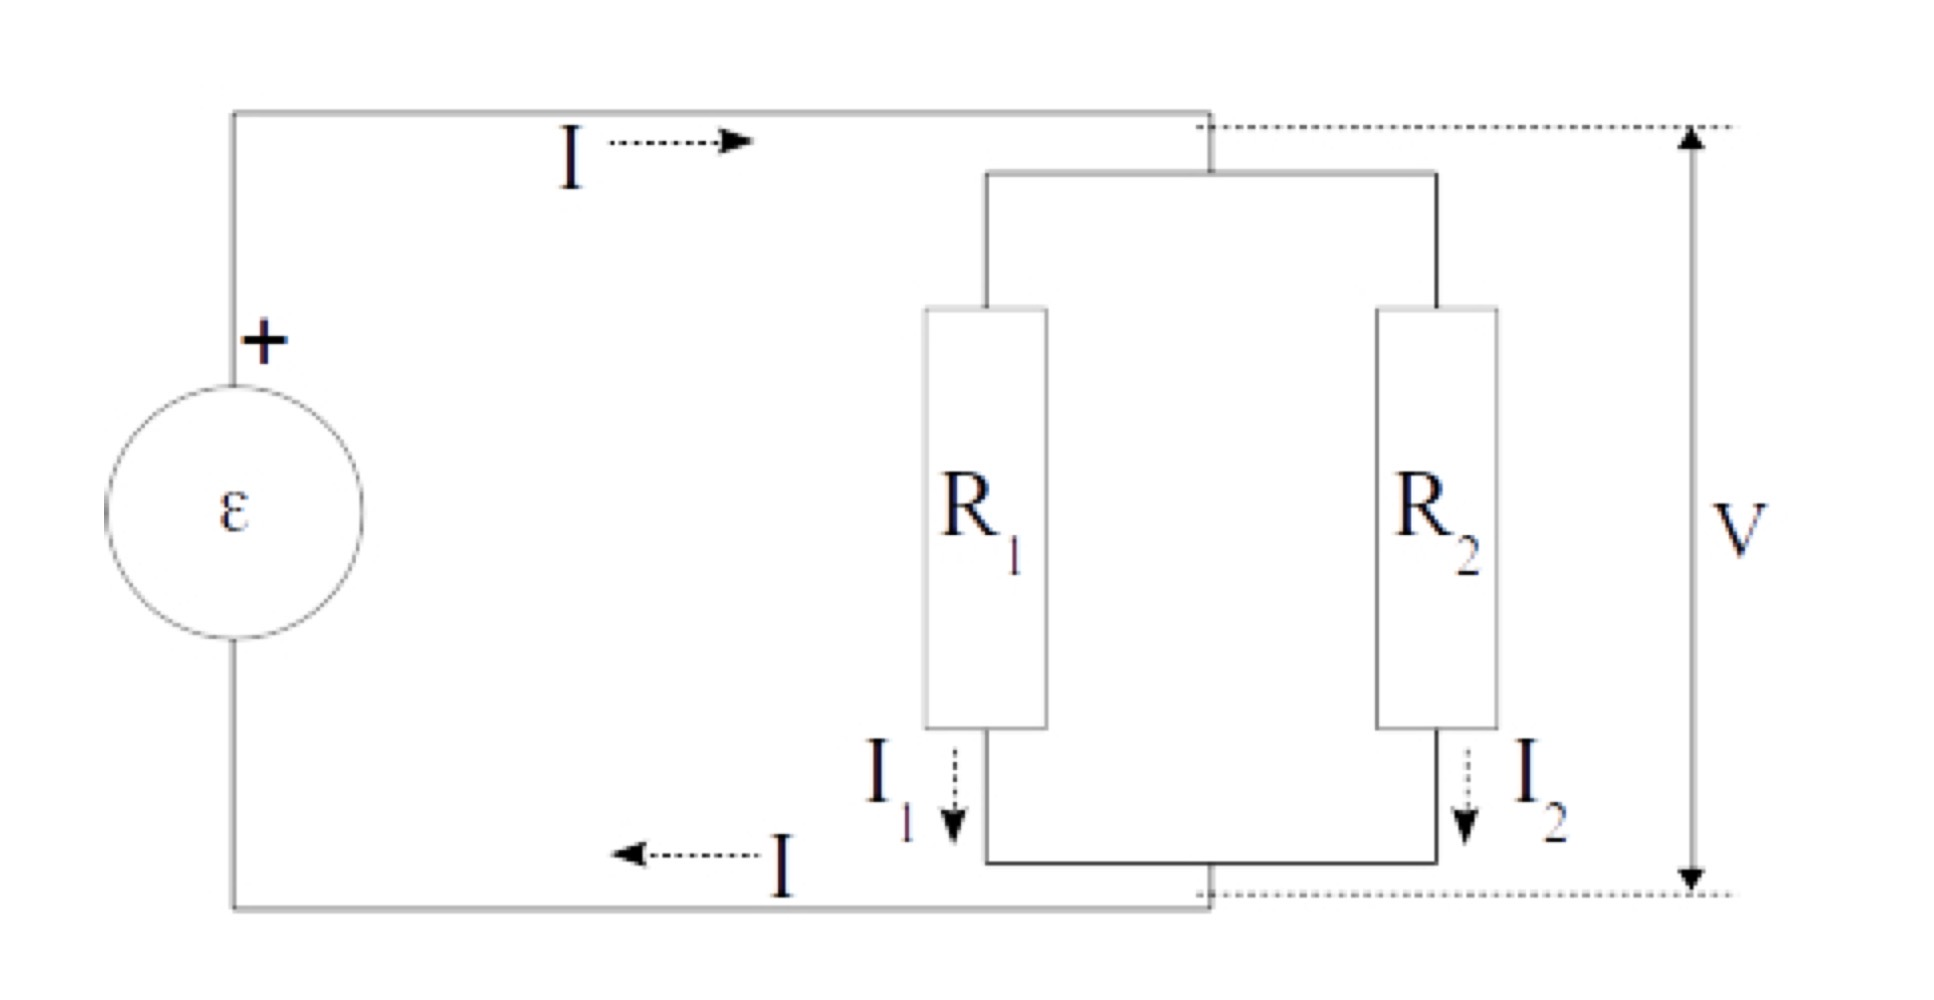
\includegraphics[width=0.7\linewidth]{continua/circuitoparalelo.jpg}
        \caption{Esquema del circuito en paralelo}
        \label{CircuitoParalelo}
    \end{figure}
    \par Como especificamos en el apartado anterior, la medida de las resistencias se realizará de forma indirecta y de forma indirecta. La medida directa se realizará conectando el polímetro al circuito, mientras que la medida indirecta se realizará igual que en el circuito en serie, con la ley de Ohm y un análisis de mínimos cuadrados
\end{itemize}

Todos estos datos experimentales vendrán acompañados por su incertidumbre, tanto para las magnitudes obtenidas de forma directa experimentalmente como para aquellas obtenidas de forma indirecta. Para la incertidumbre de las magnitudes indirectas usaremos la siguiente ecuación:

\begin{equation}
    s(y)=\sqrt{\sum_{i}\left(\frac{\partial y}{\partial x_{i}}\right)^2 s^2(x_{i})}
    \label{Incertidumbre indirecta}
\end{equation}

\subsection{Análisis de datos}

\subsubsection{Medida de resistencias}
Una vez detallada la metodología que vamos a seguir comenzaremos con la medida de las resistencias. El primer método que usaremos será el del código de colores, guiándonos por una tabla como la de la Fig.\ref{Codigo de colores}. Los datos que obtuvimos fueron los siguientes:

\begin{table}[h]
    \centering
    \begin{tabular}{|c|c|c|c|}
    \hline
    Resistencia & Valor nominal$(\Omega)$ &Tolerancia$(\%)$ & $R \pm s(R)\; (\Omega)$ \\ \hline
    $R_{1}$  &   $39\cdot 10^4$ & $\pm 5 \%$ & $39.6\cdot 10^4 \pm 2.0\cdot 10^4$\\ \hline
    $R_{2} $  &  $22 \cdot 10^4$&$\pm 5 \%$& $22 \cdot 10^4 \pm 1.1 \cdot 10^4 $ \\ \hline
    \end{tabular}
    \caption{Datos obtenidos a partir del código de colores de las resistencias}
    \label{R colores}
\end{table}

El segundo método usado para la medida de las resistencias es la medida directa con el polímetro, donde los datos obtenidos fueron los siguientes:

\begin{table}[h!]
    \centering
    \begin{tabular}{|c|c|c|c|}
    \hline
    Resistencia & Lectura$(\Omega)$ & Resolución$(\Omega)$ & $R\pm s(R)\; (\Omega)$  \\ \hline
    $R_{1}$     & $39.6\cdot 10^4$& $0.1\cdot 10^4$& $39.6 \cdot 10^4 \pm 0.1 \cdot 10^4$ \\ \hline
    $R_{2}$ & $21.9\cdot 10^4$ & $0.1\cdot 10^4$ & $21.9 \cdot 10^4 \pm 0.1 \cdot 10^4$ \\ \hline
    \end{tabular}
    \caption{Datos de la medida de resistencias con el polímetro}
    \label{R con polimetro}
\end{table}

Como podemos observar en los datos medidos con el polímetro, los valores experimentales de la resistencia están dentro del margen marcado por el fabricante en el código de colores. De esta forma corroboramos el buen funcionamiento de nuestras resistencias.
\par El último método para medir el valor de nuestras resistencias será de forma indirecta a partir de la ley de Ohm, como detallamos en la metodología. Los datos obtenidos a partir de las medidas realizadas en el circuito simple son los siguientes:

\begin{table}[ht]  %Problema con las unidades!!!!!
\begin{center}
    \begin{tabular}{|c|c|c|}
    \hline
    Medida & $V \pm s(V)$ & $I \pm s(I)(\mu A)$ \\ \hline
    $1$ & $1.08 \pm 0.01$ & $2.6 \pm 0,1$ \\ \hline
    $2$ & $2.09 \pm 0.01$ & $5.2\pm 0,1$ \\ \hline
    $3$ & $3.08 \pm 0.01$ & $7.7\pm 0,1$ \\ \hline
    $4$ & $4.04 \pm 0.01$ & $10.2\pm 0,1$ \\ \hline
    $5$ & $5.09 \pm 0.01$ & $12.8\pm 0,1 $ \\ \hline
    $6$ & $6.09 \pm 0.01$ & $15.8 \pm 0,1$\\ \hline
    $7$ & $7.05 \pm 0.01$ & $17.7\pm 0,1$ \\ \hline
    $8$ & $8.02 \pm 0.01$ & $20.2 \pm 0,1$ \\ \hline
    $9$ & $9.05 \pm 0.01$ & $22.8 \pm 0,1$ \\ \hline
    $10$ & $10.07 \pm 0.01$ & $25.3\pm 0,1$ \\ \hline
    \end{tabular}
    \captionsetup{justification=centering}  %Centrar caption
    \caption{Valores de intensidad para los diferentes voltajes con sus incertidumbres}
    \end{center}
\end{table}

\newpage

Estos datos nos van a permitir aproximar el valor de la resistencia de forma indirecta a partir de la ley de Ohm $(V=IR)$. Para ello representaremos el voltaje para diferentes intensidades y realizaremos un ajuste por el método de los mínimos cuadrados para aproximar nuestros puntos a una recta del tipo $y=bx$, donde el parámetro b (la pendiente) correspondería con el valor de la resistencia, los valores $y_{i}$ corresponden a los voltajes y los valores $x_{i}$ corresponden a las intensidades de corriente.

\begin{equation}
    b=\frac{\sum_{i}x_{i}y_{i}}{\sum_{i}x_{i}^2}=396441.9492
\end{equation}
\begin{equation}
    s=\sqrt{\frac{\sum_{i}(y_{i}-bx_{i})^2}{n-1}}=0.064
\end{equation}
\begin{equation}
    s(b)=\frac{s}{\sqrt{\sum_{i}x_{i}^2}}=0.0013
\end{equation}
\begin{equation}
    r=\frac{\sum_{i}x_{i}y_{i}}{\sqrt{(\sum_{i}x_{i}^2)(\sum_{i}y_{i}^2)}}=0.99995
\end{equation}

A partir de nuestro ajuste podemos aproximar nuestros puntos a una recta $y=bx$, que corresponde con la siguiente relación $V=RI$, siendo \newline $R=396441.9492\: \Omega$. Esto nos permite ajustar los datos a una recta de ecuación:

\begin{equation}
    V = 396441.9492 \cdot I
\end{equation}

\begin{figure}[ht]
    \centering
    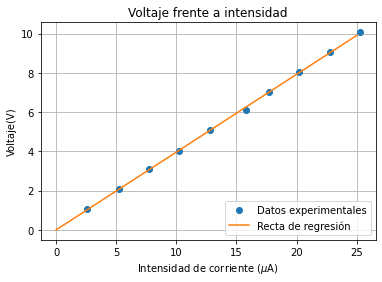
\includegraphics{continua/regresion simple.png}
    \caption{Representación del voltaje respecto a la intensidad y regresión lineal}
    \label{Regresión simple}
\end{figure}

Si comparamos los resultados obtenidos podemos observar que el valor de $39\cdot 10^4\: \Omega$ que venía establecido por el fabricante, el valor de $39.6\cdot 10^4\: \Omega$ medido con el polímetro y el valor de $39.64419492 \cdot 10^4\: \Omega$ apenas difieren menos de dos órdenes de magnitud, estando los valores experimentales dentro del límite de tolerancia. Además de eso debemos destacar la correlación entre la medida del polímetro y la obtenida a partir de la ley de Ohm, con un coeficiente de regresión muy próximo a 1 (con cuatro 9).

\newpage

\subsubsection{Medida de resistencias en serie}

El primer paso para la medida de las resistencias en serie es calcular el valor teórico, valiéndonos de la Ec.1:
    \begin{equation}    %Faltan las incertidumbres
        R_{S}=\sum_{k=1}^NR_{k}=61 \cdot 10^4 \: \Omega
    \end{equation}

La incertidumbre de esta medida indirecta se obtiene con la siguiente ecuación:
\begin{equation}
    \begin{gathered}    %Ecuación en varias líneas alineada
    s(R_{S})= \sqrt{\left (\frac{\partial R_{s}}{\partial R_{1}} \cdot s(R_{1})\right )^2+\left (\frac{\partial R_{S}}{\partial R_{2}} \cdot s(R_{2}) \right )^2}=\sqrt{(s(R_{1}))^2+(s(R_{2})^2}
    \\ s(R_{s})=2,3 \cdot 10^4 \: \Omega
    \end{gathered}
\end{equation}

Por tanto el valor de la resistencia equivalente es es el siguiente:

\begin{equation}
    R_{S} \pm s(R_{S})= 61 \cdot 10^4 \pm 2,3 \cdot 10^4 \: \Omega
\end{equation}

A continuación vamos a analizar los datos medidos del circuito con las resistencias en serie, lo primero es medir la resistencia equivalente, para la que obtuvimos un valor de $R_{S}=(61,4\pm 0.1) \cdot 10^4  \: \Omega$. Después de eso medimos los potenciales en bornes de $R_{1}$,$R_{2}$ y del conjunto de resistencias y la intensidad de corriente para 10 valores de potencial suministrados por la fuente de alimentación. Los datos obtenidos fueron los siguientes:

\begin{table}[ht]  %Faltan las incertidumbres!!!!
\centering
\begin{tabular}{|c|c|c|c|c|}
\hline
Medida & $V_{T}\pm s(V_{T})(V)$ & $V_{1} \pm s(V_{1})(V)$ & $V_{2}\pm s(V_{2})(V)$ & $I \pm s(I)(\mu A)$ \\ \hline
$1$ & $1.09\pm 0,01$ & $0.70\pm 0,01$ & $0.39\pm 0,01$ & $1.7\pm 0,1$  \\ \hline
$2$ & $2.03\pm 0,01$ & $1.31\pm 0,01$ & $0.71\pm 0,01$ & $3.3\pm 0,1$  \\ \hline
$3$ & $3.02\pm 0,01$ & $1.95\pm 0,01$ & $1.06\pm 0,01$ & $4.9\pm 0,1$  \\ \hline
$4$ & $3.99\pm 0,01$ & $2.55\pm 0,01$  & $1.44\pm 0,01$ & $6.6\pm 0,1$  \\ \hline
$5$ & $5.02\pm 0,01$ & $3.23 \pm 0,01$  & $1.79 \pm 0.01$ & $8.1 \pm 0.1$  \\ \hline
$6$ & $5.98 \pm 0.01$  & $3.84 \pm 0.01$  & $2.15 \pm 0.01$  & $9.8 \pm 0.1$  \\ \hline
$7$ & $6.93 \pm 0.01$  & $4.46 \pm 0.01$  & $2.47 \pm 0.01$  & $11.5 \pm 0.1$ \\ \hline
$8$ & $7.97 \pm 0.01$ & $5.14 \pm 0.01$  & $2.83 \pm 0.01$  & $13.1 \pm 0.1$ \\ \hline
$9$ & $8.94 \pm 0.01$  & $5.76 \pm 0.01$  & $3.18 \pm 0.01$  & $14.7 \pm 0.1$ \\ \hline
$10$ & $9.92 \pm 0,01$ & $6.39 \pm 0,01$ & $3.53 \pm 0,01$ & $16.2 \pm 0,1$ \\ \hline
\end{tabular}
\caption{Medidas del circuito con dos resistencias en serie}
\label{CircSerie}
\end{table}

\newpage A partir de los datos de $V_{T}$ y $I$ vamos a realizar una regresión lineal simple por el método de los mínimos cuadrados para aproximar el valor de la resistencia, valiéndonos de la ley de Ohm $(V=IR)$. El valor de la resistencia será la pendiente de nuestra recta de regresión, mientras que los $x_{i}$ son los valores de intensidad y los $y_{i}$ son los valores de $V_{T}$:

\begin{equation}
    b=\frac{\sum_{i}x_{i}y_{i}}{\sum_{i}x_{i}^2}=609725.7629
\end{equation}
\begin{equation}
    s=\sqrt{\frac{\sum_{i}(y_{i}-bx_{i})^2}{n-1}}=0.049
\end{equation}
\begin{equation}
    s(b)=\frac{s}{\sqrt{\sum_{i}x_{i}^2}}=0.0015
\end{equation}
\begin{equation}
    r=\frac{\sum_{i}x_{i}y_{i}}{\sqrt{(\sum_{i}x_{i}^2)(\sum_{i}y_{i}^2)}}=0.99997
\end{equation}
\newline
El valor obtenido a partir de la regresión para la resistencia es de $609725.7629 \Omega$, por lo que podemos aproximar el voltaje a la siguiente recta y hacer una representación de ambas magnitudes:
\begin{equation}
    V=609725.7629 \cdot I
\end{equation}

\begin{figure}[h!]
    \centering
    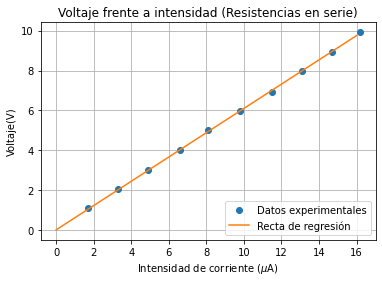
\includegraphics[width=0.75\linewidth]{continua/regresion serie.png}
    \caption{Representación del voltaje frente a la intensidad y regresión lineal en un circuito con dos resistencias en serie}
    \label{RegSerie}
\end{figure}

Una vez expuestas las medidas realizadas tanto de forma directa como de forma indirecta podemos observar una clara correlación entre las medidas y el valor teórico del conjunto de resistencias. Para el caso de la medida directa el valor teórico y el experimental difieren apenas en $0,4 \cdot 10^4 \: \Omega$, algo que entra dentro del rango de la incertidumbre del valor teórico. Para el caso de de la medida indirecta la diferencia es aún menor, de unos $275 \: \Omega$. 
\par A continuación debemos discutir la veracidad de la Ec.\ref{Formula V serie}. Para dar una cierta formalización matemática al tratamiento de estos datos, puesto que la correlación se aprecia a simple vista, vamos a calcular la media aritmética de los $V_{T}$ y de los $V_{1}+V_{2}$ y dividirlas. Cuanto más próximo esté a 1 el valor de ese cociente la correlación entre las medidas será mayor.

\begin{equation}
    \frac{\overline{V_{T}}}{\overline{V_{1}+V_{2}}}=\frac{\frac{\sum_{i}^{n}V_{Ti}}{n}}{\frac{\sum_{i}^{n}V_{1i}+V_{2i}}{n}}=\frac{\sum_{i}^{10}V_{Ti}}{\sum_{i}^{10}V_{1i}+V_{2i}}=0.9998
\end{equation}

Como podemos observar con este cálculo la correlación entre las medidas es enorme (De un $99,98\%$), por lo que podemos afirmar que se verifica la Ec.\ref{Formula V serie}.

\subsubsection{Medida de resistencias en paralelo}

Al igual que con las resistencias en serie, el primer paso en el estudio de las resistencias en paralelo es calcular el valor teórico con su incertidumbre valiéndonos de la Ec.\ref{Resistencias en paralelo} y de la Ec.\ref{Incertidumbre indirecta}:

\begin{equation}
     \frac{1}{R_{P}}=\sum_{k=1}^N\frac{1}{R_{k}} \Rightarrow \frac{1}{R_{P}}=\frac{1}{R_{1}}+\frac{1}{R_{2}} \Rightarrow R_{P}=\frac{R_{1}R_{2}}{R_{1}+R_{2}}=14.1 \cdot 10^4\: \Omega
\end{equation}

\begin{equation}
    \begin{gathered}
    s(R_{P})= \sqrt{\left (\frac{\partial R_{P}}{\partial R_{1}} \cdot s(R_{1})\right )^2+\left (\frac{\partial R_{P}}{\partial R_{2}} \cdot s(R_{2}) \right )^2} \\
    s(R_{P})=\sqrt{\left (\frac{R_{2}^2}{(R_{1}+R_{2})^2} \cdot s(R_{1})\right )^2+\left (\frac{R_{1}^2}{(R_{1}+R_{2})^2} \cdot s(R_{2}) \right )^2} \\
    s(R_{P})= 7,5 \cdot 10^3 \: \Omega
    \end{gathered}
\end{equation}

El siguiente paso es medir el conjunto de resistencias directamente en el circuito, donde obtuvimos $14,2 \cdot 10^4 \: \Omega$. Por último, medimos los potenciales en bornes del conjunto del circuito para 10 valores de potenciales suministrados por la fuente, además de la intensidad de corriente que circula por las dos resistencias y por el conjunto de ellas. Los datos obtenidos fueron los siguientes: 

\begin{table}[h!]
    \centering
    \begin{tabular}{|c|c|c|c|c|}
    \hline
    Medida & $V\pm s(V)(V)$ & $I_{1}\pm s(I_{1})(\mu A)$  & $I_{2}\pm s(I_{2})(\mu A)$   & $I_{T}\pm s(I_{T})(\mu A)$  \\ \hline
    $1$ & $1,08 \pm 0,001$ & $2,7 \pm 0,1$ & $4,7 \pm 0,1$ & $7,4 \pm 0,1$ \\ \hline
    $2$ & $2,1 \pm 0,001$ & $5,2 \pm 0,1$ & $9,6 \pm 0,1$ & $14,7 \pm 0,1$ \\ \hline
    $3$ & $3,09 \pm 0,001$ & $7,7 \pm 0,1$ & $14,0 \pm 0,1$ & $22,0 \pm 0,1$ \\ \hline
    $4$ & $4,09 \pm 0,001$ & $10,3 \pm 0,1$ & $18,6 \pm 0,1$ & $28,7 \pm 0,1$ \\ \hline
    $5$ & $5,05 \pm 0,001$ & $12,9 \pm 0,1$ & $23,2 \pm 0,1$ & $35,8 \pm 0,1$ \\ \hline
    $6$ & $6,09 \pm 0,001$ & $15,5 \pm 0,1$ & $27,6 \pm 0,1$ & $43,2 \pm 0,1$ \\ \hline
    $7$ & $7,11 \pm 0,001$ & $18,0 \pm 0,1$ & $32,1 \pm 0,1$ & $50,4 \pm 0,1$ \\ \hline
    $8$ & $8,05 \pm 0,001$ & $20,5 \pm 0,1$ & $36,7 \pm 0,1$ & $57,4 \pm 0,1$ \\ \hline
    $9$ & $9,04 \pm 0,001$ & $23,1 \pm 0,1$ & $41,5 \pm 0,1$ & $64,6 \pm 0,1$ \\ \hline
    $10$ & $10,05 \pm 0,001$ & $25,6 \pm 0,1$ & $46,1 \pm 0,1$ & $71,3 \pm 0,1$ \\ \hline
    \end{tabular}
    \caption{Medidas de potenciales e intensidades para un circuito con dos resistencias asociadas en paralelo}
    \label{Tabla paralelo}
\end{table}

A partir de los siguientes datos podemos realizar una regresión lineal, de la misma forma que en el apartado en serie, para representar el voltaje frente a la intensidad total. Obtendremos una recta de ecuación $V=bI$, donde $b$ representa el valor de la resistencia $(V=IR)$:

\begin{equation}
    b=\frac{\sum_{i}x_{i}y_{i}}{\sum_{i}x_{i}^2}=140732.62997
\end{equation}
\begin{equation}
    s=\sqrt{\frac{\sum_{i}(y_{i}-bx_{i})^2}{n-1}}=0.032
\end{equation}
\begin{equation}
    s(b)=\frac{s}{\sqrt{\sum_{i}x_{i}^2}}=0.00023
\end{equation}
\begin{equation}
    r=\frac{\sum_{i}x_{i}y_{i}}{\sqrt{(\sum_{i}x_{i}^2)(\sum_{i}y_{i}^2)}}=0.99998
\end{equation}

Los datos obtenidos a partir del análisis por mínimos cuadrados nos permiten aproximar el voltaje a una recta de regresión que tiene la siguiente ecuación:

\begin{equation}
    V = 140732.62997\cdot I
\end{equation}

A continuación podemos ver una gráfica que ilustra perfectamente la relación entre voltaje e intensidad en el circuito en paralelo:

\begin{figure}[ht]
    \centering
    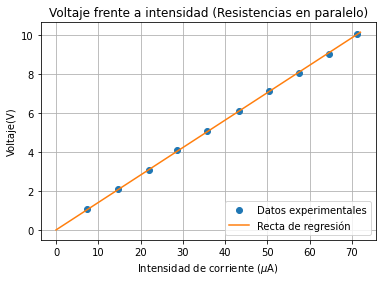
\includegraphics{continua/regresion paralelo.png}
    \caption{Medidas experimentales y recta de regresión para el circuito con dos resistencias en paralelo}
    \label{fig:my_label}
\end{figure}

\newpage Una vez expuestas las medidas directas e indirectas de la resistencia equivalente para un circuito en paralelo podemos una clara correlación entre los valores experimentales y el valor teórico. En el caso de la medida directa los valores difieren $0,1 \cdot 10^4 \: \Omega$ (dentro del valor de la incertidumbre), mientras que en la medida indirecta los valores difieren menos aún, unos $270 \: \Omega$.

\par Por último, debemos discutir también la veracidad de la Ec.\ref{Formula I paralelo}. Como realizamos en el apartado anterior con la discusión de la Ec.\ref{Formula V serie}, el formalismo matemático que realizaremos para comprobar la correlación de los datos será calcular las medias aritméticas de $I_{T}$ y de $I_{1}+I_{2}$ y dividirlas. La proximidad a 1 de ese cociente determinará el grado de correlación de los datos.

\begin{equation}
    \frac{\overline{I_{T}}}{\overline{I_{1}+I_{2}}}=\frac{\frac{\sum_{i}^{n}I_{Ti}}{n}}{\frac{\sum_{i}^{n}I_{1i}+I_{2i}}{n}}=\frac{\sum_{i}^{10}I_{Ti}}{\sum_{i}^{10}I_{1i}+I_{2i}}=0.9997
\end{equation}

Este resultado implica que el grado de correlación de las medidas es del $99,97\%$ aproximadamente, por lo que podemos confirmar la veracidad de la fórmula para la suma de intensidades.

\subsection{Conclusión}
El objetivo de esta práctica era realizar una primera aproximación al trabajo que realiza un físico en un laboratorio, en concreto comenzar a familiarizarse con el uso de elementos como el polímetro o la placa base, así como con la construcción y funcionamiento de diferentes circuitos con resistencias.

\par Comenzamos midiendo el valor de dos resistencias (con sus respectiva incertidumbre) dadas de las que desconocíamos su valor de antemano. En primer lugar obtuvimos el valor especificado por el fabricante con su rango de tolerancia interpretando su código de colores y confirmamos el valor realizando una medida de forma directa con el polímetro. Además de eso realizamos una medida de la resistencia de forma indirecta a partir de varias medidas de voltaje e intensidad en nuestro circuito simple, que nos sirvió para confirmar la ley de Ohm $(V=IR)$ realizando un ajuste por mínimos cuadrados.

\par En la última parte de la práctica estudiamos con éxito tanto un circuito con dos resistencias asociadas en serie, como otro con dos resistencias asociadas en paralelo. Medimos, con sus respectivas incertidumbres, los valores de las resistencias, confirmando así el valor teórico mediante una medida directa y otra indirecta valiéndonos de la ley de Ohm, como en el circuito simple. Además de eso confirmamos también la fórmula de suma de voltajes para el circuito en serie y la fórmula de suma de intensidades para un circuito en paralelo. 

\par Para finalizar, debemos abordar el tratamiento de incertidumbres realizado en esta práctica. Para las medidas directas hemos trabajado solamente con la incertidumbre del tipo A, para simplificar el proceso. Por otro lado en las medidas indirectas de la resistencia para los circuitos en serie y en paralelo los cálculos realizados para la propagación de errores están bien detallados en el análisis de datos.

\newpage
\subsection{Anexo: Datos utilizados para la regresión}
En este anexo serán incluidos los datos empleados en los cálculos de las regresiones lineales de forma detallada. Por comodidad expresaremos la notación científica  en formato exponencial (Ej: 2E-06$=2\cdot 10^{-6}$) 
\begin{itemize}
    \item Datos del circuito simple:
    \begin{table}[h!]
        \centering
        \begin{tabular}{|c|c|c|c|c|c|}
        \hline
        $\mathbf{x_{i}}$ & $\mathbf{y_{i}}$ & $\mathbf{x_ {i}^2}$ & $\mathbf{y_{i}^2}$ & $\mathbf{x_{i}y_{i}}$  & $\mathbf{(y_{i}-bx_{i})^2}$ \\ \hline
        2,60E-06 & 1,08  & 6,76E-12   & 1,17   & 2,81E-06 & 2,43E-03 \\ \hline
        5,20E-06 & 2,09  & 2,70E-11  & 4,37   & 1,09E-05 & 8,12E-04 \\ \hline
        7,70E-06 & 3,08  & 5,93E-11  & 9,49   & 2,37E-05 & 7,51E-04 \\ \hline
        1,02E-05 & 4,04  & 1,04E-10 & 16,32  & 4,12E-05 & 1,37E-05 \\ \hline
        1,28E-05 & 5,09  & 1,64E-10 & 25,91  & 6,52E-05 & 2,42E-04 \\ \hline
        1,58E-05 & 6,09  & 2,50E-10 & 37,09  & 9,62E-05 & 3,02E-02 \\ \hline
        1,77E-05 & 7,05  & 3,13E-10 & 49,70  & 1,25E-04 & 1,09E-03 \\ \hline
        2,02E-05 & 8,02  & 4,08E-10 & 64,32  & 1,62E-04 & 1,41E-04 \\ \hline
        2,28E-05 & 9,05  & 5,20E-10 & 81,90  & 2,06E-04 & 1,24E-04 \\ \hline
        2,53E-05 & 10,07 & 6,40E-10 & 101,40 & 2,55E-04 & 1,60E-03 \\ \hline
            &       & $\sum x_{i}^2=$2,49E-09 & $\sum y_{i}^2=$391,67  & $\sum x_{i}y_{i}=$9,88E-04 &          \\ \hline
        \end{tabular}
        \caption{Datos para los cálculos de la regresión en el circuito simple}
        \label{tab:my-table}
    \end{table}

    \item Datos del circuito en serie:
    \begin{table}[h!]
        \centering
        \begin{tabular}{|c|c|c|c|c|c|}
        \hline
        $\mathbf{x_{i}}$ & $\mathbf{y_{i}}$ & $\mathbf{x_ {i}^2}$ & $\mathbf{y_{i}^2}$ & $\mathbf{x_{i}y_{i}}$  & $\mathbf{(y_{i}-bx_{i})^2}$ \\ \hline
        1,70E-06 & 1,09 & 2,89E-12    & 1,19   & 1,85E-06 & 2,86E-03 \\ \hline
        3,30E-06 & 2,03 & 1,09E-11   & 4,12   & 6,70E-06 & 3,21E-04 \\ \hline
        4,90E-06 & 3,02 & 2,40E-11   & 9,12   & 1,48E-05 & 1,05E-03 \\ \hline
        6,60E-06 & 3,99 & 4,36E-11   & 15,92  & 2,63E-05 & 1,17E-03 \\ \hline
        8,10E-06 & 5,02 & 6,57E-11   & 25,20  & 4,07E-05 & 6,60E-03 \\ \hline
        9,80E-06 & 5,98 & 9,60E-11   & 35,76  & 5,86E-05 & 2,20E-05 \\ \hline
        1,15E-05 & 6,93 & 1,32E-10  & 48,02  & 7,97E-05 & 6,70E-03 \\ \hline
        1,31E-05 & 7,97 & 1,72E-10  & 63,52  & 1,04E-04 & 3,03E-04 \\ \hline
        1,47E-05 & 8,94 & 2,16E-10  & 79,92  & 1,31E-04 & 5,28E-04 \\ \hline
        1,62E-05 & 9,92 & 2,62E-10  & 98,41  & 1,61E-04 & 1,80E-03 \\ \hline
                 &      & $\sum x_{i}^2=$1,03E-09 & $\sum y_{i}^2=$381,19 & $\sum x_{i}y_{i}=$6,25E-04 &          \\ \hline
        \end{tabular}
        \caption{Datos para los cálculos de la regresión lineal en el circuito en serie}
        \label{tab:my-table}
    \end{table}

    \newpage
    \item Datos del circuito en paralelo:

    \begin{table}[h!]
        \centering
        \begin{tabular}{|c|c|c|c|c|c|}
        \hline
        $\mathbf{x_{i}}$ & $\mathbf{y_{i}}$ & $\mathbf{x_ {i}^2}$ & $\mathbf{y_{i}^2}$ & $\mathbf{x_{i}y_{i}}$  & $\mathbf{(y_{i}-bx_{i})^2}$   \\ \hline
        7,40E-06 & 1,08  & 5,48E-11 & 1,17   & 7,99E-06 & 1,49E-03 \\ \hline
        1,47E-05 & 2,10   & 2,16E-10 & 4,41     & 3,09E-05 & 9,75E-04 \\ \hline
        2,20E-05 & 3,09  & 4,84E-10 & 9,55   & 6,80E-05 & 3,74E-05 \\ \hline
        2,87E-05 & 4,09  & 8,24E-10 & 16,73  & 1,17E-04 & 2,60E-03 \\ \hline
        3,58E-05 & 5,05  & 1,28E-09 & 25,50  & 1,81E-04 & 1,39E-04 \\ \hline
        4,32E-05 & 6,09  & 1,87E-09 & 37,09  & 2,63E-04 & 1,07E-04 \\ \hline
        5,04E-05 & 7,11  & 2,54E-09 & 50,55  & 3,58E-04 & 2,92E-04 \\ \hline
        5,74E-05 & 8,05  & 3,29E-09 & 64,80  & 4,62E-04 & 7,87E-04 \\ \hline
        6,46E-05 & 9,04  & 4,17E-09 & 81,72  & 5,84E-04 & 2,63E-03 \\ \hline
        7,13E-05 & 10,05 & 5,08E-09 & 101,00 & 7,17E-04 & 2,48E-04 \\ \hline
                 &       & $\sum x_{i}^2=$1,98E-08 & $\sum y_{i}^2=$392,52 & $\sum x_{i}y_{i}=$2,79E-03 &          \\ \hline
        \end{tabular}
        \caption{Datos para los cálculos de la regresión del circuito en paralelo}
        \label{tab:my-table}
\end{table}

\end{itemize}


\newpage

\section{Corriente alterna}
\subsection{Objetivos}
\begin{itemize}
    \item Familiarizarse con el uso de un osciloscopio digital, así como con el manejo de circuitos de corriente alterna
    \item Obtener los parámetros característicos de un circuito de corriente alterna, como la frecuencia de corte, la impedancia o la reactancia capacitiva
 
\end{itemize}


\subsection{Materiales y metodología}
\begin{itemize}
    \item Placa base y cables de conexión
    \item Resistencia (10k$\Omega$) y condensador (12k pF)
    \item Generador de señales (fuente de fem senoidal
    \item Osciloscopio digital
\end{itemize}

Para llevar a cabo nuestro experimento lo primero que haremos es construir un circuito muy básico con la resistencia y el condensador, conectados en serie, además de nuestro generador de señales. Este circuito nos servirá para medir los potenciales en bornes de la fuente, la resistencia y el condensador para los diferentes valores de frecuencia, como se muestra en la Fig.1 y en la Fig.2.


\begin{figure}[ht]
    \begin{subfigure}{0.5\textwidth}
        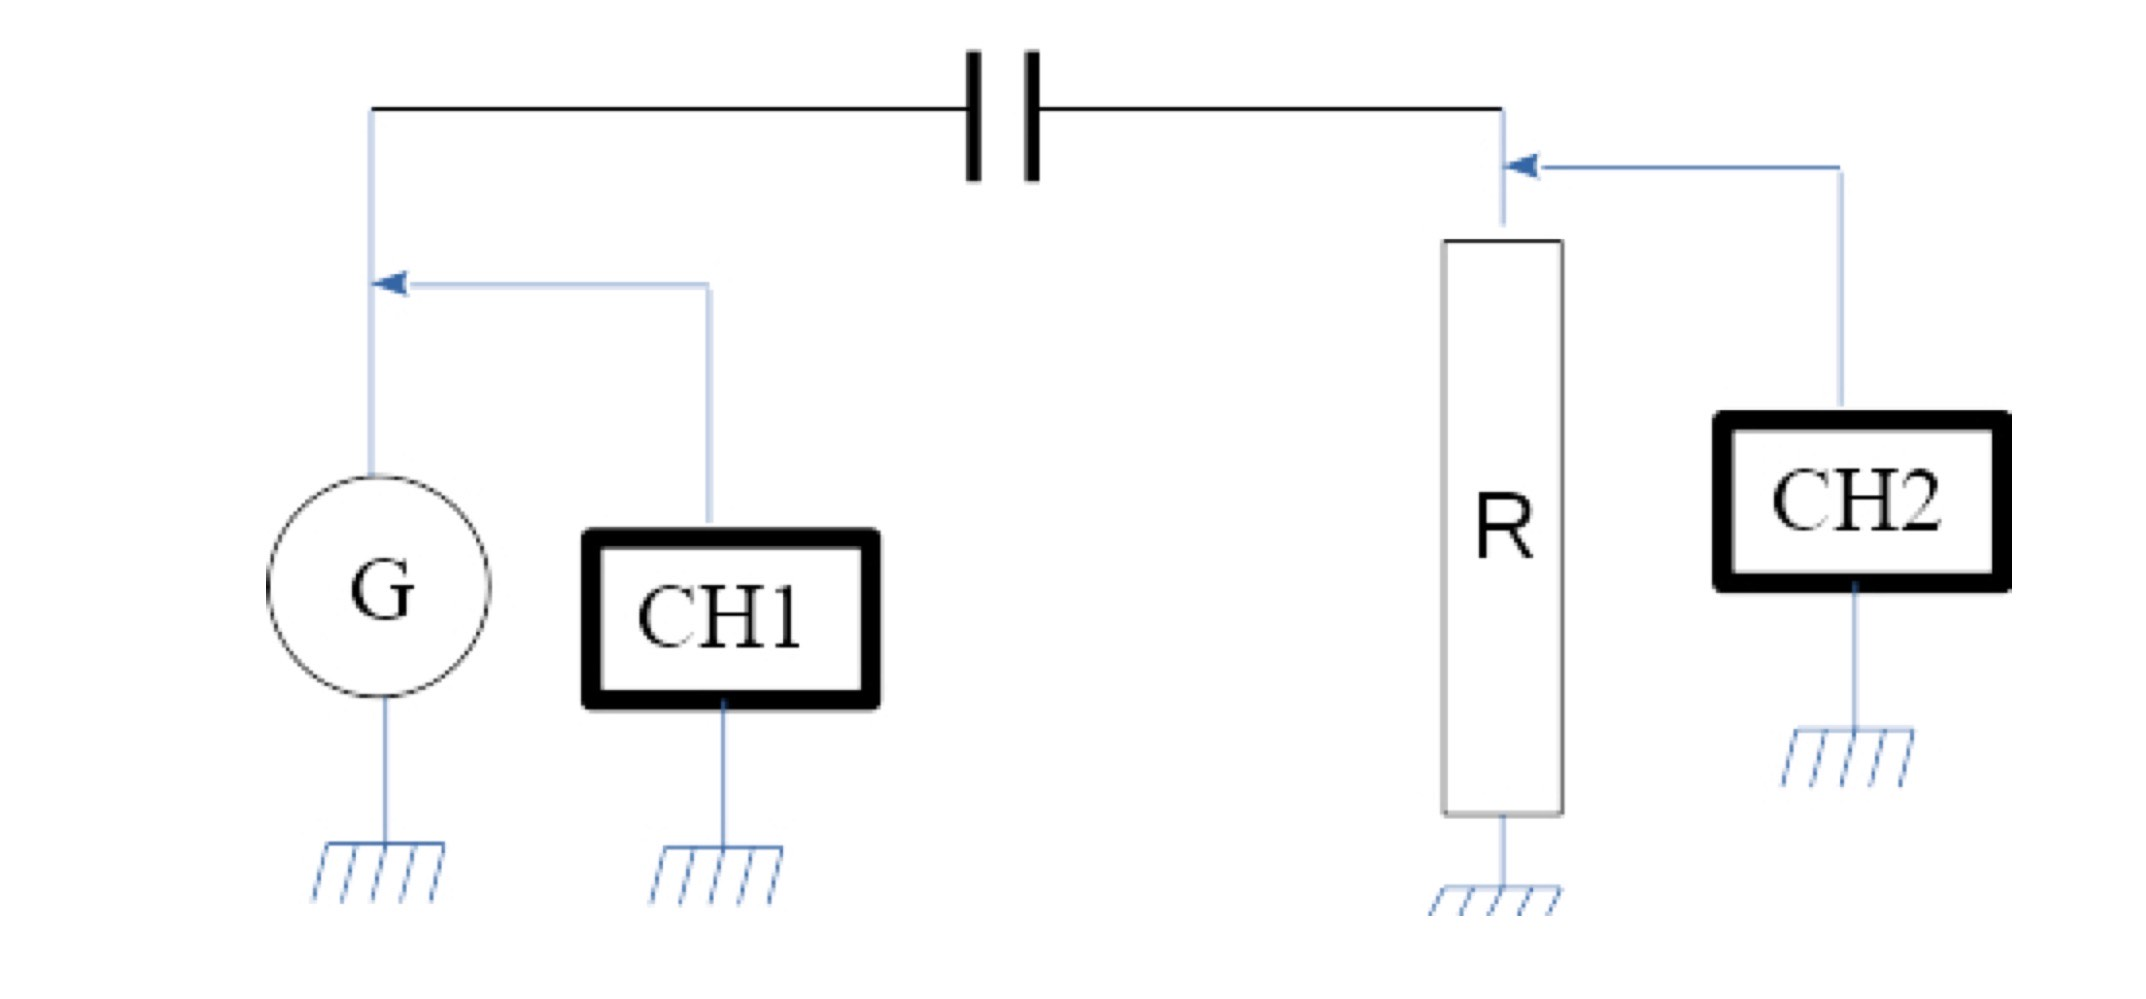
\includegraphics[width=0.9\linewidth]{alterna/potencialresistencia.jpg}
        \caption{Circuito para medir $V_{m}$ y $V_{mR}$}
        \label{Vm y Vmr}
    \end{subfigure}
    \begin{subfigure}{0.5\textwidth}
        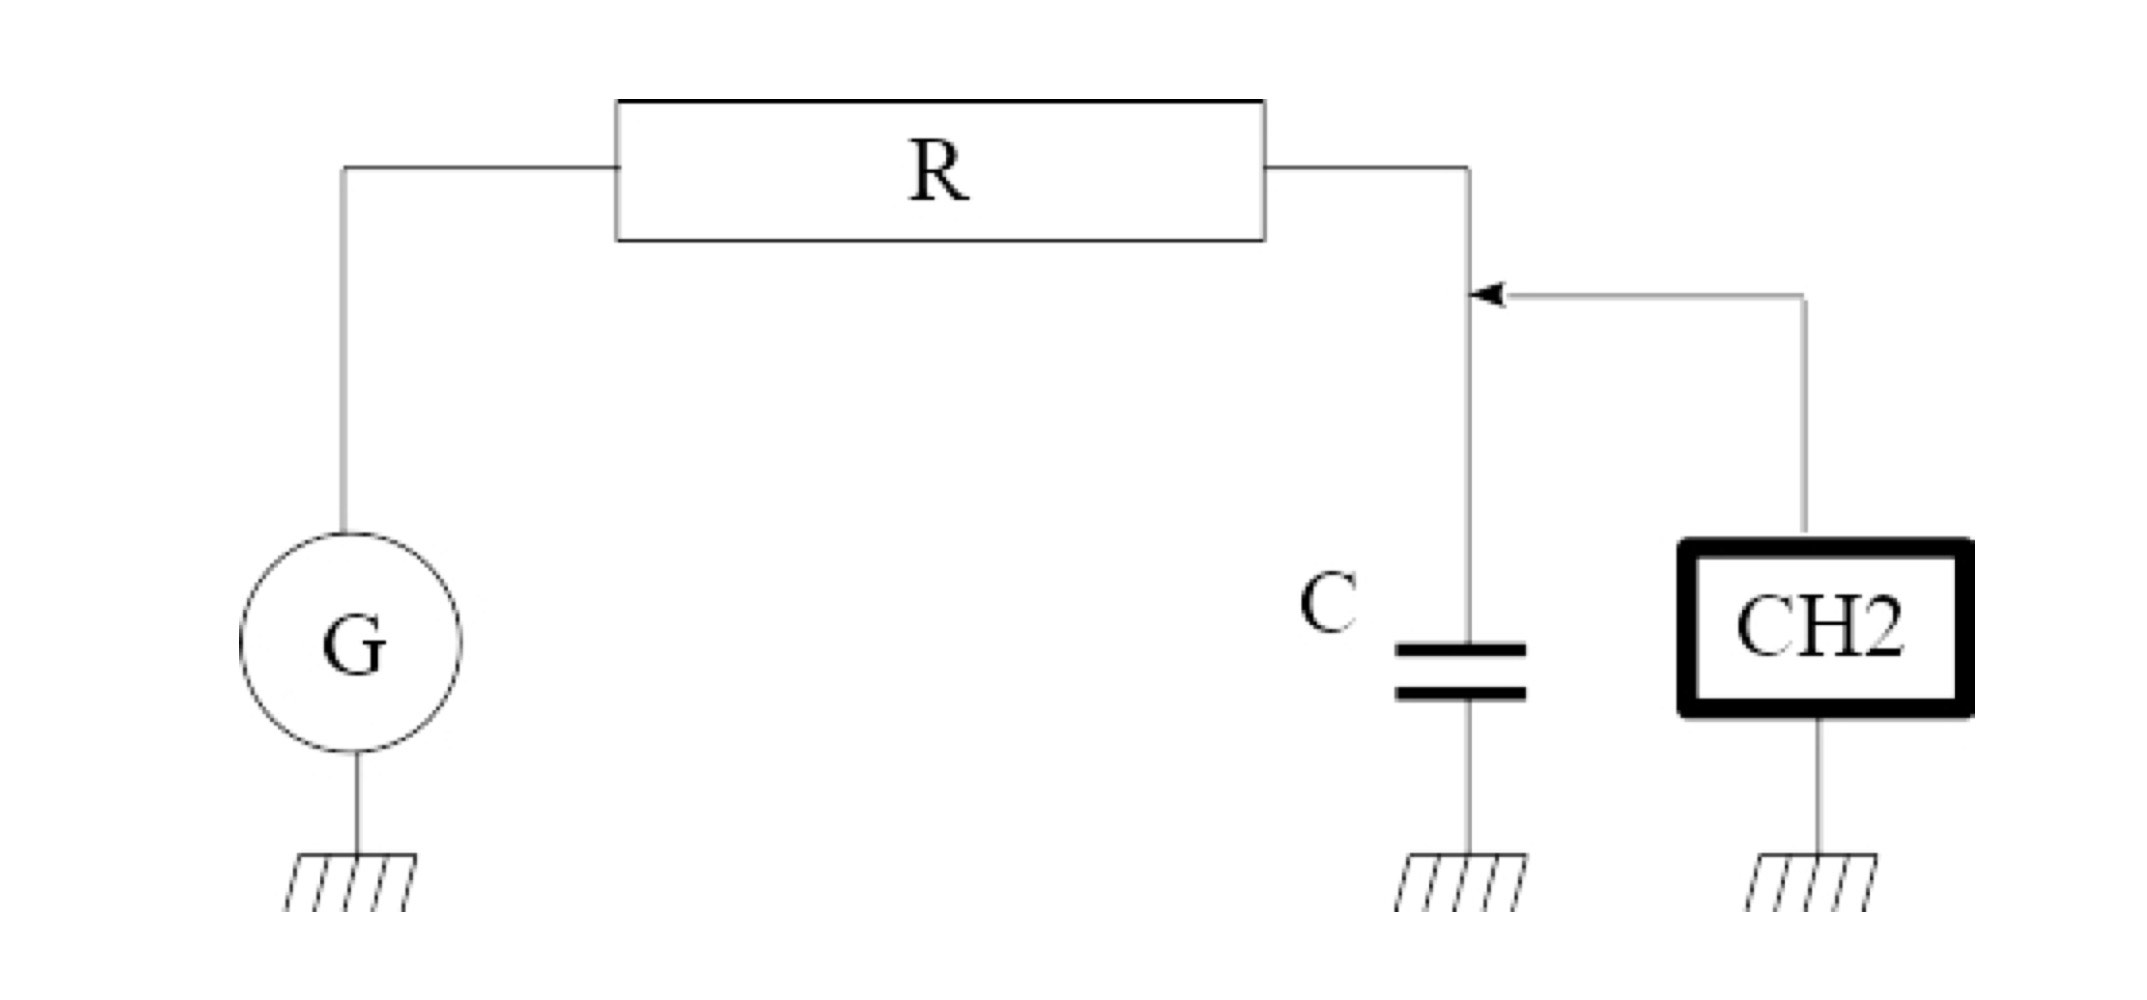
\includegraphics[width=0.9\linewidth]{alterna/potencialcondensador.jpg}
        \caption{Circuito para medir$V_{mC}$}
        \label{Vmc}
    \end{subfigure}
\caption{Esquemas de los circuitos realizados}
\label{Esquemas circuitos}
\end{figure}

Los datos de los potenciales calculados experimentalmente nos serán útiles para el cálculo de la impedancia $(Z)$, magnitud que representaremos frente a la frecuencia para hacer una estimación de la frecuencia de corte, como se demostrará en el siguiente apartado.

\newpage
\par    %Nuevo párrafo
La última parte de la práctica consiste en medir el desfase entre que existe entre las señales del generador $(V_{G})$ y de la resistencia $(V_{R})$. Para ello volveremos al primer circuito de la Fig.\ref{Esquemas circuitos} y mediremos los diferentes $\Delta t$ con el osciloscopio en modo dual. Los valores de $t_{1}$ y $t_{2}$ se fijan cuando las señales cruzan el eje horizontal, como se muestra en la Fig.\ref{Desfase}.

\begin{figure}[h]
    \centering
    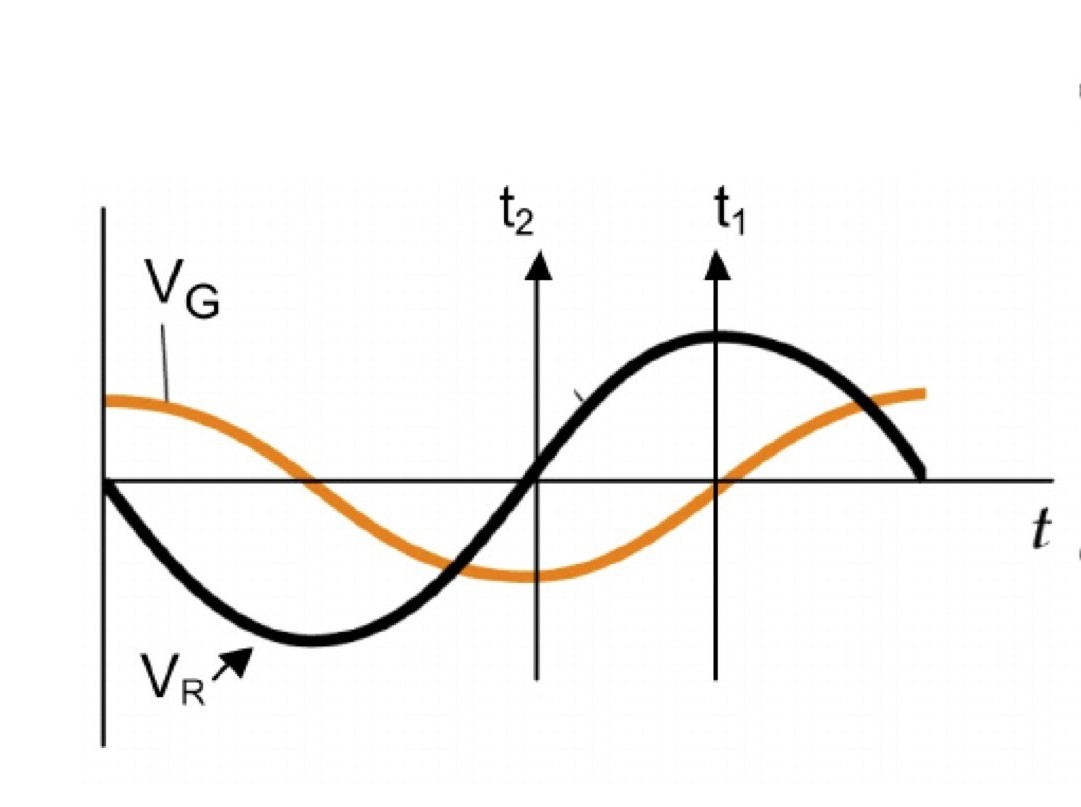
\includegraphics[width=0.6\linewidth]{alterna/desfase2.jpg}
    \caption{Representación del desfase entre señales}
    \label{Desfase}
\end{figure}


\subsection{Análisis de datos}
\subsubsection{Frecuencia de corte}

Para llevar a cabo el análisis de nuestros datos experimentales el primer paso es calcular el valor teórico de la frecuencia de corte, sustituyendo los valores de R y C:

\begin{equation}
    \label{fc}
    f_{C}=\frac{1}{2\pi RC} \Rightarrow f_{C}=\frac{1}{2\pi \cdot 10^4 \cdot 12 \cdot 10^{-9}} = 1326,29\: Hz %Espacio pequeño
\end{equation}

Ahora vamos a calcular el valor de la constante de tiempo del circuito, que será una aproximación del valor real, puesto que no conocemos los datos de incertidumbre del condensador y de la fuente generadora de señales:

\begin{equation}
    \label{ConstanteT}
    T=RC=10^4 \cdot 12 \cdot 10^{-9}=1,2 \cdot 10^{-4}\: s
\end{equation}

Una vez calculado el valor teórico de la $f_{C}$ vamos a compararlo con el valor que obtendremos a partir de nuestros datos experimentales de los potenciales en bornes de los diferentes elementos del circuito. \newline


\begin{table}[ht]
    \begin{center}
    \resizebox{10cm}{!}{
    \begin{tabular}[h]{|c| c| c| c| c| c|}
        \hline
        \boldmath{$f(Hz)$} & \boldmath{$\log_{10}f$} & \boldmath{$V_{m}(V)
        $} & \boldmath{$V_{mR}(V)$} & \boldmath{$V_{mC}(V)$} & \boldmath{$V_{mR}/V_{mC}$}\\ \hline
          300 & 2,477 & 9 & 1,95 & 8,40 & 0,23 \\ \hline 
          400 & 2,602 & 9 & 2,52 & 8,20 & 0,31\\ \hline
          500 & 2,699 & 9 & 3,04 & 8,00 & 0,38 \\ \hline
          600 & 2,778 & 9 & 3,60 & 7,80 & 0,46 \\ \hline
          700	& 2,845 & 9 &	4,08 &	7,40 &	0,55 \\ \hline
          800 &	2,903 &	9 &	4,56 &	7,20 &	0,63 \\ \hline
          900 &	2,954 &	9 &	4,88 &	7,00 &	0,70 \\ \hline
          1000&	3&	9&	5,28&	6,80&	0,78 \\ \hline
          1100& 3,041&9&5,52&	6,40&0,86\\ \hline
          1200&	3,079&	9&	5,81&	6,20&	0,94 \\ \hline
          1350&	3,130&	9&	6,08&	6,00&	1,01 \\ \hline
          1400&	3,146&	9&	6,16&	5,80&	1,06 \\ \hline
          1500&	3,176&	9&	6,40&	5,40&	1,19 \\ \hline
          1700&	3,230&	9&	6,72&	5,20&	1,29 \\ \hline
          2000&	3,301&	9&	7,12&	4,80&	1,48 \\ \hline
          2400&	3,380&	9&	7,52&	4,40&	1,71 \\ \hline
          2900&	3,462&	9&	7,84&	4,20&	1,87 \\ \hline
          3500&	3,544&	9&	8,00&	3,80&	2,10 \\ \hline
          3750&	3,574&	9&	8,08&	3,60&	2,24 \\ \hline
          3999&	3,602&	9&	8,16&	3,40&	2,40\\ \hline
    \end{tabular}
    }
    \captionsetup{justification=centering}  %Centrar caption
    \caption{Medidas de los potenciales en bornes de la fuente, la resistencia y el condensador}
    \end{center}
\end{table}

Para estimar la frecuencia de corte experimentalmente debemos representar la impedancia (Z) frente a la frecuencia (ambas magnitudes en escala logarítmica), en una gráfica RC. Esta gráfica constará de tres curvas:
\begin{itemize}
    \item La curva RC
    \item La curva R, que representará el valor de la resistencia frente a la frecuencia
    \item La curva C, que representará a la reactancia capacitiva frente a la frecuencia
\end{itemize}
Estas dos últimas curvas serán asíntotas de la curva RC y su intersección debería coincidir con el valor teórico de la frecuencia de corte.
\par Para nuestra representación necesitamos conocer los valores de la impedancia y la reactancia capacitiva para frecuencia en escala logarítmica:

\begin{equation}
    \label{Imepedancia y capacitancia}
    Z=R(\frac{V_{R}}{V_{mR}}) \; \; \; X_{C}=\frac{1}{\omega C} \; \; \; \omega = 2\pi f \; \Rightarrow \; X_{C}=\frac{1}{2\pi fC}
\end{equation}

\begin{table}[ht]
    \centering
    \resizebox{10cm}{!}{
    \begin{tabular}{|c|c|c|c|c|c|}
        \hline
         \boldmath{$f(Hz)$} & \boldmath{$log_{10}f$} & \boldmath{$Z(\Omega)$} & \boldmath{$20\log Z$} & \boldmath{$X_{C}(\Omega)$} & \boldmath{$20\log X_{C}$} \\ \hline
        300&	2,477&	46153,85&	93,28&	44209,71&	92,91\\ \hline
        400&	2,602&	35714,29&	91,06&	33157,28&	90,41\\ \hline
        500&    2,699&	29605,26&	89,43&	26525,82&	88,47\\ \hline
        600&	2,778&	25000,00&	87,96&	22104,85&	86,89\\ \hline
        700&    2,845&	22058,82&	86,87&	18947,02&	85,55\\ \hline
        800&	2,903&	19736.84&	85,91&	16578,64&	84,39\\ \hline
        900&    2,954&	18442,62&	85,32&	14736,59&	83,37\\ \hline
        1000&	3,000&	17045,45&	84,63&	13262,91&	82,45\\ \hline
        1100&	3,041&	16304,35&	84,25&	12057,19&	81,62\\ \hline
        1200&	3,079&	15490,53&	83,80&	11052,43&	80,87\\ \hline
        1350&	3,130&	14802,63&	83,41&	9824,34	 &   79,85\\ \hline
        1400&	3,146&	14610,39&	83,30&	9473,51	  &  79,53\\ \hline
        1500&	3,176&	14062,50&	82,96&	8841,94	   & 78,93\\ \hline
        1700&	3,230&	13392,86&	82,54&	7801,71	    &77,84\\ \hline
        2000&	3,301&	12640,45&	82,03&	6631,46&	    76,43\\ \hline
        2400&	3,380&	11968,09&	81,56&	5526,21	&    74,85\\ \hline
        2900&	3,462&	11479,59&	81,20&	4573,42	 &   73,20\\ \hline
        3500&	3,544&	11250,00&	81,02&	3789,40	  &  71,57\\ \hline
        3750&	3,574&	11138,61&	80,94&	3536,78	   & 70,97\\ \hline
        3999&	3,602&	11029,41&	80,85&	3316,56	  &  70,41\\ \hline
    \end{tabular}
    }
    \caption{Cálculo de la impedancia y la reactancia capacitiva}
    \label{Tab2}
\end{table}

El valor teórico de la frecuencia de corte es de 1326,29 Hz, que debería coincidir con el punto de corte de las curvas R y C. Para calcularlo analíticamente necesitamos conocer la ecuación de ambas curvas. La ecuación de la curva R se obtiene de forma trivial, pues la resistencia tiene un valor constante de 10k$\Omega$. Para ello debemos calcular el valor de $20\log_{10}(R)$:

\begin{equation}
    20\log_{10}(R)=20\log_{10}(10.000)=80,00
\end{equation}

Por tanto la ecuación de la curva R es $y=80$. Para conocer la ecuación de la curva C tendremos que hacer una aproximación por el método de los mínimos cuadrados a partir de los datos de la reactancia capacitiva. Con eso obtendremos una recta del tipo $y=a+bx$, con la que podremos calcular la intersección.
\begin{equation}
    20\log X_{C}=a+b\log(f)
\end{equation}

% Mínimos cuadrados con TI
\begin{equation}
    a=\frac{(\sum_{i}y_{i})(\sum_{i}x_{i}^2)-(\sum_{i}x_{i})(\sum_{i}x_{i}y_{i})}{n(\sum_ix_{i}^2)-(\sum_{i}x_{i})^2}=142.45277771188293
\end{equation}
\begin{equation}
    b=\frac{n(\sum_{i}x_{i}y_{i})-(\sum_{i}x_{i})(\sum_{i}y_{i})}{n(\sum_{i}x_{i}^2)-(\sum_{i}x_{i})^2}=-19.999999999999496
\end{equation}
\begin{equation}
    s=\sqrt{\frac{\sum_{i}(y_{i}-a-bx_{i})^2}{n-2}}=7,7 \cdot 10^{-13}
\end{equation}
\begin{equation}
    s(a)=s\sqrt{\frac{\sum_{i}x_{i}^2}{n(\sum_{i}x_{i}^2)-(\sum_{i}x_{i})^2}}=1,7 \cdot 10^{-12}
\end{equation}
\begin{equation}
    s(b)=s\sqrt{\frac{n}{n(\sum_{i}x_{i}^2)-(\sum_{i}x_{i})^2}}=5,4 \cdot 10^{-13}
\end{equation}

\begin{equation}
    r=\frac{n(\sum_{i}x_{i}y_{i})-(\sum_{i}x_{i})(\sum_{i}y_{i})}{\sqrt{[n(\sum_{i}x_{i}^2)-(\sum_{i}x_{i})^2][n(\sum_{i}y_{i}^2)-(\sum_{i}y_{i}^2)-(\sum_{i}y_{i})^2]}}=-0.99999999999996
\end{equation}

Obtenemos así la ecuación aproximada de la curva C, de la forma:
\begin{equation}
    y=142.45277771188293-19.999999999999496x
\end{equation}

Para obtener el valor de $\log_{10}f$ en donde las curvas R y C interseccionan debemos resolver la siguiente ecuación:

\begin{equation}
    80=142.45277771188293-19.999999999999496x
\end{equation}
Al resolverla obtenemos un valor de $x=3,12264$, que corresponde con un valor para la frecuencia de corte de $10^{3,12264}=1326,294596\: Hz$, muy similar al calculado teóricamente.

\par Por último, cabe destacar que el coeficiente de regresión tiene un valor negativo por ser $X_{C}$ y la frecuencia magnitudes inversamente proporcionales.
\newpage

\begin{figure}[h!]
    \centering
    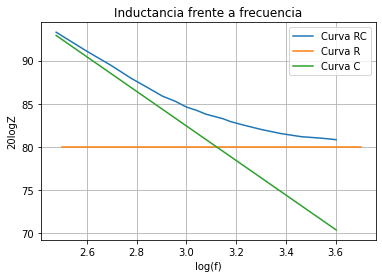
\includegraphics[width=0.9\linewidth]{alterna/CurvaRC.png}
    \caption{Curvas RC, R y C}
    \label{CurvaRC}
\end{figure}

Para terminar con nuestro cálculo de la frecuencia de corte a partir de los datos experimentales vamos a representar la función $\frac{V_{mR}}{V_{mC}}$   respecto a la frecuencia. Para ello vamos a realizar un ajuste lineal por el método de los mínimos cuadrados de los datos obtenidos, aproximando nuestros datos a una recta del tipo $y = bx$, ya que no tenemos término independiente. El valor de la frecuencia de corte se corresponde con la frecuencia que verifique que $\frac{V_{mR}}{V_{mC}}=1$.

% Mínimos cuadrados sin TI
\begin{equation}
    b=\frac{\sum_{i}x_{i}y_{i}}{\sum_{i}x_{i}^2}=0.0006555746874182195
\end{equation}
\begin{equation}
    s=\sqrt{\frac{\sum_{i}(y_{i}-bx_{i})^2}{n-1}}=0.14315488119093
\end{equation}
\begin{equation}
    s(b)=\frac{s}{\sqrt{\sum_{i}x_{i}^2}}=1.6437544976917146 \cdot 10^{-5}
\end{equation}
\begin{equation}
    r=\frac{\sum_{i}x_{i}y_{i}}{\sqrt{(\sum_{i}x_{i}^2)(\sum_{i}y_{i}^2)}}=0.994
\end{equation}
\newline

A partir de nuestro análisis por mínimos cuadrados podemos aproximar nuestros datos de $\frac{V_{mR}}{v_{mC}}$ a una recta de ecuación:
\begin{equation}
    y=0.0006555746874182195x
\end{equation}

\begin{figure}[h]
    \centering
    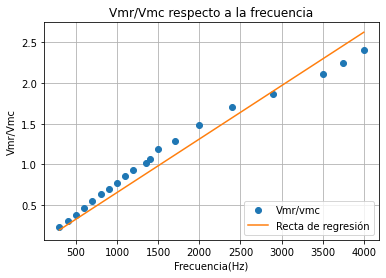
\includegraphics{alterna/regresionVmRvsVmC.png}
    \caption{Representación de $\frac{V_{mR}}{V_{mC}}$ frente a la frecuencia}
    \label{Vmr/Vmc}
\end{figure}

 El valor de la frecuencia de corte coincide con el valor de frecuencia para el que $\frac{V_{mR}}{V_{mC}}=1$, es decir:

 \begin{equation}
     1=0.0006555746874182195x
 \end{equation}

 Si resolvemos esta ecuación obtenemos un valor para la frecuencia de corte de $x = 1525.379211845708\: Hz$, algo mayor que el valor teórico $(1326,29\: Hz)$. Esta discordancia se debe probablemente a un error a la hora de realizar las mediciones, que es sustancialmente mayor al error cometido en el método de las curvas R y C (se puede observar por los coeficientes de regresión, siendo el del primer método mucho más próximo a 1).

\newpage

 \subsubsection{Desfase entre señales}
La otra parte de la práctica consiste en medir el desfase que existe entre las señales del generador $(V_{G})$ y de la resistencia $(V_{R})$. Para ello debemos medir $\Delta t$ entre las dos señales para los diferentes valores de frecuencia, pues ambas magnitudes están relacionadas mediante la siguiente fórmula:

\begin{equation}
    \varphi=-2\pi f\Delta t
\end{equation}

Donde $\varphi$ es la diferencia de fase de las señales de $V_{G}$, de fase $\omega t_{1}$, y $V_{R}$, de fase $\omega t_{2}+\varphi$.

\begin{table}[h]
    \centering
    \begin{tabular}{|c|c|c|c|c|}
        \hline
        \boldmath{$f(Hz)$}&\boldmath{$\log_{10}f$}&\boldmath{ $\Delta t(\mu s)$}&\boldmath{$\varphi (rad)$}&\boldmath{$\varphi ($º$)$}\\ \hline
        300&	 2,477&	680&	1,282&	73,45\\ \hline
        400	&    2,602&	520&	1,206&	69,10\\ \hline
        500	&    2,699& 360&	1,131&	64,80\\ \hline
        600	&    2,778&	320&	1,206&	69,10\\ \hline
        700	&    2,845&	240&	1,056&	60,50\\ \hline
        800	&    2,903&	200&	1,005&	57,58\\ \hline
        900	&    2,954&	164&	0,927&	53,11\\ \hline
        1000&	3,000&	152&	0,955&	54,72\\ \hline
        1100&	3,041&	128&	0,885&	50,7\\ \hline
        1200&	3,079&	104&	0,784&	44,92\\ \hline
        1350&	3,130&	88&	0,764&	43,77\\ \hline
        1400&	3,146&	84&	0,739&	42,34\\ \hline
        1500&	3,176&	72&	0,679&	38,9\\ \hline
        1700&	3,230&	60&	0,641&	36,73\\ \hline
        2000&	3,301&	48&	0,603&	34,55\\ \hline
        2400&	3,380&	32&	0,482&	27,62\\ \hline
        2900&	3,462&	28&	0,510&	29,22\\ \hline
        3500&	3,544&	20&	0,440&	25,21\\ \hline
        3750&	3,574&	16&	0,377&	21,60\\ \hline
        3999&	3,602&	12&	0,302&	17,30\\ \hline

    \end{tabular}
    \caption{Medidas de $\Delta t$ y cálculo del desfase}
    \label{Tabla desfase}
\end{table}

A partir de los datos obtenidos experimentalmente podemos representar gráficamente el desfase (en grados sexagesimales), frente a la frecuencia\newline (en escala logarítmica). El valor de la frecuencia de corte debería coincidir con un valor de $\varphi = 45º$. Para calcular el valor del desfase a partir de nuestros datos los hemos ajustado al siguiente polinomio de orden tres mediante Python:

\begin{equation}
    y=50.388x^3-464.717x^2+1364.764x-1220.366
\end{equation}

\begin{figure}[h]
    \centering
    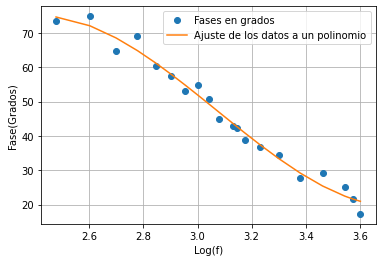
\includegraphics{alterna/faseVSfrecuencia.png}
    \caption{Representación del desfase frente a la frecuencia en escala logarítmica}
    \label{FaseVSfrecuencia}
\end{figure}

Para calcular analíticamente el valor aproximado de la frecuencia de corte a partir de nuestro polinomio de grado 3 tenemos que resolver la siguiente ecuación:
\begin{equation}
    45=50.388x^3-464.717x^2+1364.764x-1220.366
\end{equation}
\par Esta ecuación tiene dos raíces reales, pero nos interesa solo la que se encuentra en nuestro rango de frecuencias, $x=3,10892$. La frecuencia asociada a ese valor es:
\begin{equation}
    10^{3,10892}=1285,0499232\: Hz
\end{equation}
\par Este valor de la frecuencia de corte se acerca bastante al calculado teóricamente, de $1326,29 \:Hz$, el error se debe seguramente a la aproximación por el polinomio y a los errores a la hora de tomar las medidas experimentales.

\newpage

\subsection{Conclusión}
El objetivo de esta práctica era realizar una primera aproximación al tratamiento de circuitos de corriente alterna, entendiendo la corriente eléctrica como una oscilación. Además de eso tuvimos la oportunidad de tratar por primera vez con instrumentos de medida, como el osciloscopio, o nuevos elementos para la construcción de circuitos eléctricos, como el condensador.

\par Como conclusión podemos afirmar que hemos comprobado experimentalmente el valor de la frecuencia de corte con los dos métodos propuestos, mediante la intersección de las curvas R y C y mediante la representación del cociente $\frac{V_{mR}}{V_{mC}}$ para los diferentes valores de frecuencia. Además de eso pudimos medir los diferentes desfases entre la señal del generador y de la resistencia para cada valor de frecuencia, comprobando con bastante éxito que el desfase para la frecuencia de corte es de $45\degree$.

\end{document}
